\subsection{Compilation remainder}

\begin{frame}
\frametitle{Compilation remainder}

\begin{itemize}
	\item understanding the different compilation phases
	\item what are {\tt Makefiles} ?
	\item what happen to the application when using the different optimization flags ? 
\end{itemize}

\end{frame}

\subsection{Back to the roots}

\begin{frame}
\frametitle{{\tt 00111001011100110111...}}

{\bf Back to the roots}

\begin{itemize}
%	\item a computer (in fact a processor or a CPU) understands nothing but {\bf ON} and {\bf OFF} (one or zero)
	\item a computer (in fact a processor or a CPU) understands nothing but {\bf ON} and {\bf OFF} ({\tt 1} or {\tt 0})
	\item There is a 4-stages process to transform a {\bf source code} from a programming language into {\it something} which is understandable by the processor (the {\bf Machine Code})
\end{itemize}

\end{frame}


\begin{frame}
\frametitle{Programming languages}

Different programming languages :

\begin{itemize}
	\item {\bf C/C++} or {\bf Fortran} are high level compiled languages
%	\item {\bf Matlab}, {\bf Python}, {\bf R} are high level interpreted languages
\end{itemize}

they are {\bf human readable} % and with a {\bf high level of abstraction}

\begin{itemize}
	\item The {\bf assembly language} (depending on the CPU) is a {\bf low level language}
\end{itemize}

difficult to read. It calls only CPU instructions like a LOAD, a jump or a numerical operation.

\begin{itemize}
	\item the {\bf machine code} (depending on the CPU) is the only {\bf language understandable by the processor}
\end{itemize}

\end{frame}

\begin{frame}
\frametitle{Compilation}
\begin{alertblock}{Question}
How to produce machine code out of high-level language ? For instance from a {\tt C} source code ?
\end{alertblock}
\end{frame}

\begin{frame}
\frametitle{Punch cards}
\begin{center}
{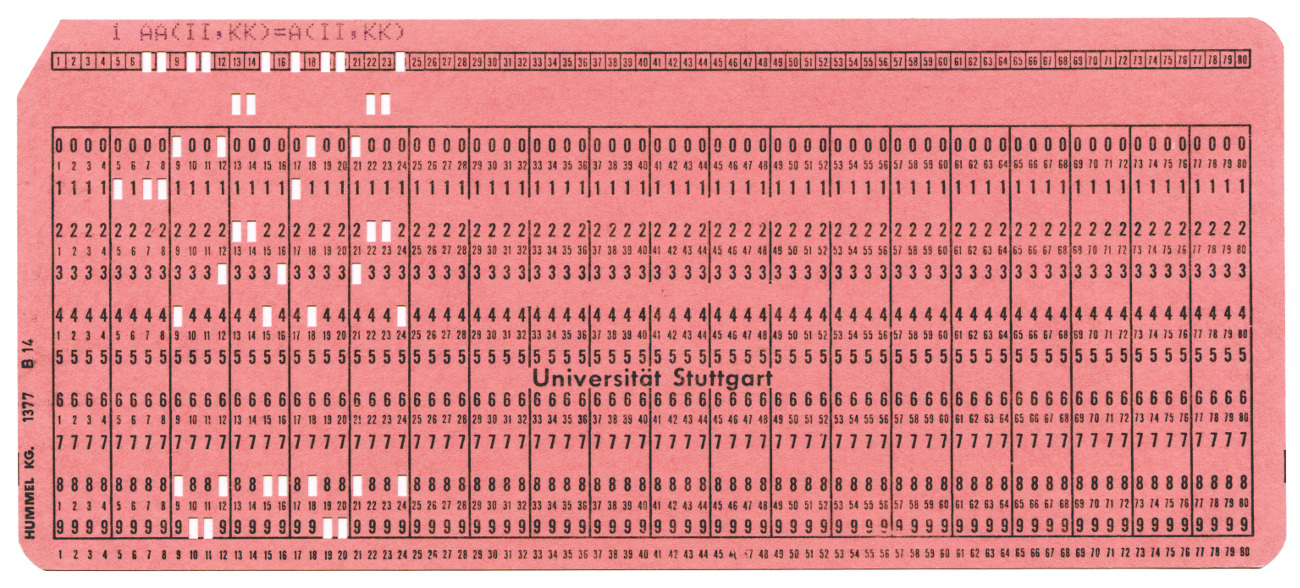
\includegraphics[width=11cm]{Day2/images/punch-card.jpg}}
\end{center}
\end{frame}

\begin{frame}
\frametitle{Modern days : with a compiler}
\begin{center}
{% Slide 34
\begin{tikzpicture}

\node[stage] (Preproc) at (0,0) {\stagename{Preprocessor} \texttt{gcc -E file.c -o file.i}};
\node[stage] (Compiler) at (0,-2) {\stagename{Compiler} \texttt{gcc -S file.i -o file.s}};
\node[stage] (Assembler) at (0,-4) {\stagename{Assembler} \texttt{gcc -c file.s -o file.o}};
\node[stage] (Linker) at (0,-6) {\stagename{Linker} \texttt{gcc file.o -lexample -o file}};

\node[stage highlight, right of = Assembler, yshift = -1cm, xshift = 5cm, minimum width = 4cm] (Lib) {\stagename{External library} libexample.so};


\draw[->] (Preproc) -- (Compiler);
\draw[->] (Compiler) -- (Assembler);
\draw[->] (Assembler) -- (Linker);
\draw[->, dashed] (Lib.west) -- (Linker.east);

\end{tikzpicture}
}
\end{center}
\end{frame}


\begin{frame}[containsverbatim]
\frametitle{Example with a C source}
\begin{lstlisting}[language=C,frame=lines]
#include <stdio.h>
#include <stdlib.h>
#define up 10
int main() {
   int i,n;
   n = 0;
   for (i = 0; i < up; i++){
      n = n + 1;
   }
   return 0;
}
\end{lstlisting}

\url{https://gcc.godbolt.org/}

\end{frame}


\begin{frame}[containsverbatim]
\frametitle{Preprocessor ({\tt gcc -E})}
\begin{verbatim}
(...)
# 1 "/usr/include/x86_64-linux-gnu/bits/stdlib-float.h" 1 3 4
# 956 "/usr/include/stdlib.h" 2 3 4
# 968 "/usr/include/stdlib.h" 3 4

# 3 "very-simple.c" 2

int main() {
 int i,n;
 n = 0;
 for (i = 0;i < 10; i++){
  n = n + 1;
 }
 return 0;
}
\end{verbatim}
\end{frame}


\begin{frame}[containsverbatim]
\frametitle{Compiler ({\tt gcc -S})}
\begin{verbatim}
main:
.LFB2:
      pushq     %rbp
      movq      %rsp, %rbp
      movl      $0, -8(%rbp)
      movl      $0, -4(%rbp)
      jmp       .L2
.L3:
      addl      $1, -8(%rbp)
      addl      $1, -4(%rbp)
.L2:
      cmpl      $9, -4(%rbp)
      jle       .L3
      movl      $0, %eax
      popq      %rbp
      ret
\end{verbatim}
\end{frame}



\begin{frame}[containsverbatim]
\frametitle{Assembler ({\tt gcc -c})}
\begin{verbatim}
   0:	55                   	push   %rbp
   1:	48 89 e5             	mov    %rsp,%rbp
   4:	c7 45 f8 00 00 00 00 	movl   $0x0,-0x8(%rbp)
   b:	c7 45 fc 00 00 00 00 	movl   $0x0,-0x4(%rbp)
  12:	eb 08                	jmp    1c <main+0x1c>
  14:	83 45 f8 01          	addl   $0x1,-0x8(%rbp)
  18:	83 45 fc 01          	addl   $0x1,-0x4(%rbp)
  1c:	83 7d fc 09          	cmpl   $0x9,-0x4(%rbp)
  20:	7e f2                	jle    14 <main+0x14>
  22:	b8 00 00 00 00       	mov    $0x0,%eax
  27:	5d                   	pop    %rbp
  28:	c3                   	retq   
\end{verbatim}
(using {\tt objdump -d file.o})
\end{frame}


\begin{frame}[containsverbatim]
\frametitle{Linker ({\tt gcc -o})}
\begin{alertblock}{}
This last stage produces the actual executable (by linking against external libraries if required)
\end{alertblock}
\end{frame}


\begin{frame}[containsverbatim]
\frametitle{All stages in one command}

\begin{itemize}
	\item In real life, it is very unusual that one go through all the stages separatly.
	\item The two main phases are {\bf compilation} ({\tt gcc -c}) and {\bf linking} ({\tt gcc -o})
\end{itemize}

\begin{verbatim}
vkeller@deneb1:~]$ gcc -c file1.c -o file1.o
vkeller@deneb1:~]$ gcc -c file2.c -o file2.o
vkeller@deneb1:~]$ gcc file1.o file2.o -o app.exe
vkeller@deneb1:~]$ ./app.exe
\end{verbatim}

\begin{itemize}
	\item or both at once :
\end{itemize}

\begin{verbatim}
vkeller@deneb1:~]$ gcc file1.c file2.c -o app.exe
vkeller@deneb1:~]$ ./app.exe
\end{verbatim}
\end{frame}

\begin{frame}
\frametitle{But ...}

\begin{itemize}
	\item complexity whith multiple files
	\item dependencies
	\item need for a more complex tool : {\tt Makefiles} !
\end{itemize}
\end{frame}


\subsection{Makefile}

\begin{frame}
\frametitle{About Makefiles}

\begin{itemize}
	\item a {\tt Makefile} is nothing but a {\bf recipe} on how to produce an executable
		\begin{itemize}
			\item what to compile ?
			\item how to compile ?
			\item what to link ?
			\item how to link ?
		\end{itemize}
	\item useful for large projects or for testing purpose
	\item full (re)usage of {\tt variables}
	\item The usual name is {\tt Makefile} or {\tt makefile} or specified when calling {\tt make -f special.makefile}
\end{itemize}
\end{frame}

\begin{frame}[containsverbatim]
\frametitle{What is contained in a Makefile ?}
As an example
\begin{itemize}
	\item a source file {\tt poisson.c} to compile
	\item you want to produce two executable versions : 
	\begin{itemize}
		\item non-optimized with debug information
		\item optimized 
	\end{itemize}
	\item with the GNU compiler
\end{itemize}

\begin{verbatim}
gcc -O0 -g poisson.c -lm -o p-gcc-debug.exe
gcc -O3 -ftree-vectorize poisson.c -lm -o p-gcc-optim.exe
\end{verbatim}
\end{frame}

\begin{frame}[containsverbatim]
\frametitle{What is contained in a Makefile ?}
\begin{verbatim}
CC       = gcc
CFLAGS   = -O3 -ftree-vectorize
LDFLAGS  = -lm

all: p-gcc-optim.exe

.o.c: 
     $(CC) -c $(CFLAGS) $(OBJ) $<
OBJ = poisson.o

p-gcc-optim.exe: 
     $(CC) $(LDFLAGS) $(OBJ) -o $@

clean:
     rm -f *.o p-gcc-optim.exe
\end{verbatim}
\end{frame}

\begin{frame}[containsverbatim]
\frametitle{How to use the Makefile ?}

to get the optimized version :
\begin{verbatim}
make
\end{verbatim}

to get the non-optimized with debug information version :
\begin{verbatim}
make CFLAGS="-O0 -g"
\end{verbatim}

Optimized version with the Intel compiler ?
\begin{verbatim}
make CC=icc CFLAGS="-O3 -xHost" LDFLAGS=""
\end{verbatim}

or by editing the variables {\tt CC}, {\tt CFLAGS} and {\tt LDFLAGS} in the Makefile.

\end{frame}


\subsection{Optimization flags}


\begin{frame}
\frametitle{Compiler optimization}

\begin{itemize}
	\item Different levels of optimization
	\begin{itemize}
		\item instructions level
		\item datatype level
		\item global level (inter-procedural optimization or ''IPO'')
		\item loops level
		\item machine code optimization
	\end{itemize}
	\item it is possible to optimize at each level
	\item {\bf Optimization by compiler can lead to semantic changes} thus wrong results ! 
\end{itemize}

\end{frame}


\begin{frame}
\frametitle{Compiler optimization}

\begin{itemize}
	\item {\tt gcc -O0} no optimization
	\item {\tt gcc -O1} ''the compiler tries to reduce code size and execution time''
	\item {\tt gcc -O2} ''performs nearly all supported optimizations that do not involve a space-speed tradeoff''
	\item {\tt gcc -O3} ''optimize yet more. It is -O2 plus others''. Warning: this can change the code semantics.
	\item {\tt gcc -Ofast} ''Disregard strict standards compliance.''
	\item {\tt gcc -ftree-vectorize} ''perform vectorization on trees enables all -O3 optimizations plus -ffast-math''
\end{itemize}

\end{frame}





